\documentclass[12pt]{report}

\usepackage{setspace}
\renewcommand{\baselinestretch}{1.5}
\usepackage{float}
\usepackage{lipsum}
\usepackage{graphicx}
\usepackage{subcaption}
\usepackage[table,xcdraw,dvipsnames]{xcolor}
\usepackage{titlesec}
\usepackage{titletoc}
\usepackage{titling}
\usepackage[T1]{fontenc}
\usepackage[utf8x]{inputenc}
\usepackage{amsmath}
\usepackage{caption}
%\usepackage[a4paper,margin=0.5in]{geometry}
\usepackage[a4paper,%
            left=2cm,right=2cm,top=1cm,bottom=1cm,%
            footskip=.25in]{geometry}
\usepackage[normalem]{ulem}
\usepackage[none]{hyphenat}
\usepackage[hidelinks]{hyperref}
\PassOptionsToPackage{hyphens}{url}\usepackage{hyperref}
\useunder{\uline}{\ul}{}

% No hyphenation (word wrapping) with text justification
\tolerance=1
\emergencystretch=\maxdimen
\hyphenpenalty=10000
\hbadness=10000

% Replace table caption name
\usepackage{caption}
\captionsetup[table]{name=Tableau}

% For toc, lot and lof
\usepackage[titles]{tocloft}

% Liste des figures et les tableaux!
\graphicspath{{figures/}}
\usepackage{array}

% Disable auto indentation globally
\setlength{\parindent}{0pt}

% Choix de Font Family!
\usepackage{mathptmx}
%\usepackage{tgtermes}
%\usepackage{tgpagella}
%\usepackage{helvet}
%\usepackage{tgbonum}

% fancy logo for page numbers!
\usepackage{fancyhdr,blindtext,tikz}
\usepackage{lastpage,refcount}

% Box frame for figures #\fbox{}
\setlength{\fboxsep}{0pt}
\setlength{\fboxrule}{3pt}

% Options: Sonny, Lenny, Glenn, Conny, Rejne, Bjarne, Bjornstrup
\usepackage[Conny]{fncychap}

% Redifining from 0.1 to 1 ... 2 ... and so on
\renewcommand{\thesection}{\arabic{section}}

% Renaming Bibliography name
\renewcommand\bibname{Bibliographie}

% Bibliography styling
\bibliographystyle{plain}

% Redifining from 1.1 to 1.a ... 1.b ... and so on
%\renewcommand{\thesubsection}{\alph{subsection}}

% Pour enlever les nombres dans le TOC pour les Chapitres
\titlecontents{part}[1em]
{\vskip 0.5ex\bfseries\large}%
{}% numbered sections formatting
{\itshape\scshape}% unnumbered sections formatting
{}%

% Pour enlever les nombres dans le TOC pour les Chapitres
\titlecontents{chapter}[1em]
{\vskip 0.5ex\bfseries\large}%
{}% numbered sections formatting
{\itshape\scshape}% unnumbered sections formatting
{\titlerule*[0.3pc]{.}\contentspage}%

% Pour les section aussi
\titlecontents{section}[1em]
{\vskip 0.2ex\bfseries\large}%
{\hspace{0.15in}\contentslabel{0.13in}.\hspace{0.1in}}% numbered sections formatting
{\itshape}% unnumbered sections formatting
{\titlerule*[0.3pc]{.}\contentspage}%

% Pour les subsection
\titlecontents{subsection}[3.5em]
{\large}%
{\contentslabel{0.10in}.\hspace{0.25in}}% numbered sections formatting
{}% unnumbered sections formatting
{\titlerule*[0.3pc]{.}\contentspage}%

% Custom colors!
\definecolor{MYCOL}{HTML}{00318A}

% List of Figures settings:
\renewcommand{\listfigurename}{Liste Des Figures}
\renewcommand{\cftloftitlefont}{\vspace*{-0.6in}\hfill\color{Blue}\fontsize{35}{43}\bfseries}
\renewcommand{\cftafterloftitle}{\hfill}
\setlength{\cftfigindent}{0pt} % left aligned Fig entries
\renewcommand{\cftfigpresnum}{Figure } % put before the number
\renewcommand{\cftfigaftersnum}{:} % put before the number
\addtolength{\cftfignumwidth}{2.5em} % extra space for \cftpresnum

% List of Tables settings:
\renewcommand{\listtablename}{Liste Des Tableaux}
\renewcommand{\cftlottitlefont}{\vspace*{-0.6in}\hfill\color{Blue}\fontsize{35}{43}\bfseries}
\renewcommand{\cftafterlottitle}{\hfill}
\setlength{\cfttabindent}{0pt} % left aligned Tab entries
\renewcommand{\cfttabpresnum}{Tableau } % put before the number
\renewcommand{\cfttabaftersnum}{:} % put before the number
\addtolength{\cfttabnumwidth}{2.5em} % extra space for \cftpresnum

% Table of contents settings:
\renewcommand{\contentsname}{Table Des Matières}

\usepackage[framemethod=TikZ]{mdframed}

% Pour la box de Th\`eme!
\mdfdefinestyle{MyFrame}{%
    linecolor=black,
    outerlinewidth=6pt,
    roundcorner=12pt,
    innertopmargin=13pt,
    innerbottommargin=13pt,
    innerrightmargin=20pt,
    innerleftmargin=20pt,
    backgroundcolor=gray!30!white}


% My custom page style
\fancypagestyle{myfancy}{%   
   \fancyhf{}%
   \fancyfoot[C]{\tikz[baseline={(0,0)},anchor=center] \node[label={center:\thepage}]{
\includegraphics[scale=.037]{../images/cloud.png}};}%
   \renewcommand{\headrulewidth}{0pt}%
   \renewcommand{\footrulewidth}{0pt}%
   \fancyhead{}
   \fancyfoot{}
   \fancyfoot[C]{\vspace{-0.35in}\textcolor{Gray}{\Large{Page}}\hspace{0.04in} \large{\thepage}\hspace{0.07in}\large{|}\hspace{0.07in}\large{\pageref{LastPage}}}
}%
\pagestyle{empty}

% Custom environment
\newenvironment{changemargin}[2]{%
\begin{list}{}{%
\setlength{\topsep}{0pt}%
\setlength{\leftmargin}{#1}%
\setlength{\rightmargin}{#2}%
\setlength{\listparindent}{\parindent}%
\setlength{\itemindent}{\parindent}%
\setlength{\parsep}{\parskip}%
}%
\item[]}{\end{list}}

% 'myfancy' page styling is also applied on chapters!
\usepackage{etoolbox}
\patchcmd{\chapter}{\thispagestyle{empty}}{\thispagestyle{myfancy}}{}{}

\titleformat{\chapter}
{\centering\fontsize{40}{50}\bfseries\color{Blue}\scshape}
{}
{}
{\vspace{-1.7in}{\color{Blue} \rule{\linewidth}{1.2mm} }}[\vspace{-0.35in}{\color{Blue} \rule{\linewidth}{1.2mm} }\vspace{-1in}]

\titleformat{\section}
{\Large\bfseries\color{MidnightBlue}}
{\thesection.\hspace{0.08in}}
{0em}
{}[\titlerule]

\titleformat{\subsection}
{\large\bfseries\color{RoyalBlue}}
{\hspace{0.25in}\thesubsection\hspace{0.08in}}
{0em}
{}[]

\titleformat{\subsubsection}
{\bfseries\large}
{\hspace{0.40in}}
{0em}
{}[]

\newenvironment{myindentpar}[1]%
  {\begin{list}{}%
          {\setlength{\leftmargin}{#1}}%
          \item[]%
  }
  {\end{list}}

\usepackage{tikz}
\usetikzlibrary{calc}

\begin{document}

\begin{titlepage}

   \begin{tikzpicture}[remember picture, overlay]
      \draw[line width = 2pt] ($(current page.north west) + (0.25in,-0.25in)$) rectangle ($(current page.south east) + (-0.25in,0.25in)$);
   \end{tikzpicture}

   \begin{center}
       \vspace*{-0.4in}

       \begin{large}

           République Algérienne Démocratique et Populaire

           Ministère de l'Enseignement Supérieur et de la Recherche Scientifique

           Université M'Hamed Bougara de Boumerdès

       \end{large}

       \vspace{0.1in}

    \begin{figure}[h]
    \centering
        
\includegraphics[width = 1.5in, height = 1in]{../images/UnivUMBB.jpg}
    \end{figure}
     \vspace*{-0.1in}
    \large{Faculté des Sciences}
    \\
    \vspace*{-0.1in}
    \large{Département d'informatique}
   \end{center}

    \hspace{0.2in}
    \large{\textbf{Domaine \,\; :}  Mathématiques Informatique}
    \kern 1in
    \large{\textbf{Année universitaire :}}

    \hspace{0.2in}
    \large{\textbf{Filière \quad\,\,\, :}  Informatique}
    \kern 2.65in
    2021 / 2022

    \hspace{0.2in}
    \large{\textbf{Spécialité \, :}  Technologie de l'information}

    \begin{center}
        \begin{large}

            \vspace{0.1in}

            \textit{\textbf{\uline{Mini projet pour le module technologie des composants}}}
        
        \end{large}

        \vspace{0.3in}

        \textit{\Huge{\textbf{\uline{Thème}}}}

        \vspace{0.2in}

        \begin{mdframed}[style=MyFrame]
            \begin{center}
            \color{BlueViolet}
              \LARGE{\textbf{Application de réservation d'hôtel}}

              \LARGE{\textbf{utilisant NextJS}}
            \end{center}
        \end{mdframed}
    \end{center}

    \vspace{0.4in}

    \hspace{0.2in}
    \textit{\textbf{Présenté par :}}

    \hspace{0.2in}
    Boudraa Mohamed Ouadjih

    \hspace{0.2in}
    Bakiri Insaf

    \hspace{0.2in}
    Neggazi Mohamed Lamine

\end{titlepage}

\newpage

\vspace*{0.2in}

\thispagestyle{empty}

\begin{center}
    {\color{Blue} \rule{3in}{1.4mm} }\\
    \vspace{0.1in}
    \scshape{\fontsize{34}{46}{\bfseries{\color{Blue}{Résumé}}}}
    \\
    \vspace{0.6in}
\end{center}
\cftaddtitleline{toc}{part}{\vspace{-0.12in}\color{Blue}{Résumé}}{}
\begin{changemargin}{0.9cm}{0.9cm}
\hspace*{0.16in}
Il existe de nombreuses technologies qui sont utilisées sur Internet pour partager des fichiers, chacune d’entre elles ont des fonctionnalités, des méthodes et des protocoles différents. Cependant, le plus commun et le plus facile est le Web qui a été établi par quelques fonctionnalités simples. Le Web se développe continuellement pour être aussi facile pour les utilisateurs. Les développeurs Web veulent créer une machine qui pense comme des humains en ajoutant de nouveaux outils, méthodes et protocoles au Web actuel.
\\\\
\hspace*{0.16in}
L’objectif de cet article est de présenter NextJS, l’un des frameworks les plus populaires qui aide les développeurs du monde entier à créer des sites Web, et également de présenter notre exemple de site Web créé par NextJS et hébergé par Vercel.
\\\\
\hspace*{0.16in}
Le résultat final n’est pas le site Web lui-même, mais plutôt l’expérience de développement dans laquelle les développeurs bénéficieront le plus, "La vérité ne peut être trouvée qu’à un seul endroit: le code.". \textsuperscript{\cite{martin2018clean}}
\end{changemargin}

\vspace{1in}

\begin{changemargin}{0.9cm}{0.9cm}
Mots clés : Internet, Web, NextJS, Vercel, code.
\end{changemargin}

\newpage

\vspace*{0.2in}

\thispagestyle{empty}

\begin{center}
    {\color{Blue} \rule{3in}{1.4mm} }\\
    \vspace{0.1in}
    \scshape{\fontsize{34}{46}{\bfseries{\color{Blue}{Abstract}}}}
    \\
    \vspace{0.6in}
\end{center}
\cftaddtitleline{toc}{part}{\vspace{-0.12in}\color{Blue}{Abstract}}{}
\begin{changemargin}{0.9cm}{0.9cm}
\hspace*{0.16in}
There are many technologies which are used on the Internet to share files, each of them have different features, methods and protocols. However, the most common and easiest one is the Web which was established by a few simple features. The Web continuously developing to be as much as easy for the users. Web developers want to make a machine which thinks like humans by adding new tools, methods and protocols to the current Web.
\\\\
\hspace*{0.16in}
The objectif of this paper is to showcase NextJS, one of the most popular frameworks that helps developers around the world create websites, and also showcase our sample website created by NextJS and hosted by Vercel.
\\\\
\hspace*{0.16in}
The final outcome is not the website itself, but rather the development experince in which developers will benefit the most, "Truth can only be found in one place: the code.". \textsuperscript{\cite{martin2018clean}}
\end{changemargin}

\vspace{1in}

\begin{changemargin}{0.9cm}{0.9cm}
Keywords: Internet, Web, NextJS, Vercel, code.
\end{changemargin}

\newpage

\cftaddtitleline{toc}{part}{\vspace{-0.12in}\color{Blue}{Table des matières}}{}
\tableofcontents

\newpage

\cftaddtitleline{toc}{part}{\vspace{-0.12in}\color{Blue}{Liste des figures}}{}
\listoffigures

\newpage

\cftaddtitleline{toc}{part}{\vspace{-0.12in}\color{Blue}{Liste des tableaux}}{}
\listoftables

\addtocontents{toc}{\protect\renewcommand{\protect\cftsecleader}{\protect\cftdotfill{\protect\cftsecdotsep}}}

\addtocontents{lof}{\protect\thispagestyle{empty}}
\addtocontents{lot}{\protect\thispagestyle{empty}}
\addtocontents{toc}{\protect\thispagestyle{empty}}

\newpage

\pagestyle{myfancy}

\vspace*{-0.2in}

\setcounter{page}{1}

\begin{center}
    {\color{Blue} \rule{6.2in}{1.4mm} }\\
    \vspace{0.1in}
    \scshape{\fontsize{34}{46}{\bfseries{\color{Blue}{Introduction générale}}}}
    \\
    \vspace{0.5in}
\end{center}
\addcontentsline{toc}{chapter}{\vspace{-0.12in}\color{Blue}{Introduction générale}}
\hspace*{0.16in}
Au dernier siècle, L'internet devient de plus en plus important pour nous les humains, car il est utilisé littéralement pour tout ce que nous faisons, nous y accédons quotidiennement pour faire diverses activités telles que faire des achats, communiquer, vérifier la map...Et pour cela on a besoin de sites Web pour faire de telles choses.
\\\\
\hspace*{0.16in}
De nos jours, le développement d'un site web est un parcours long et compliqué, il est à la fois coûteux et difficile pour les développeurs d'en créer un. Le développement Web a vu un énorme avènement de l’application à page unique (SPA) au cours des deux dernières années. Le développement initial était simple : rechargez une page complète pour effectuer une modification de l’affichage ou effectuer une action de l’utilisateur. Le problème avec cela était un énorme temps d’aller-retour pour la demande complète pour atteindre le serveur Web et revenir au client.
\\\\
\hspace*{0.16in}
C’est dans ce contexte, le NextJS offre une excellente expérience utilisateur, une facilité d’utilisation et un fractionnement automatique du code qui profite aux développeurs débutants et avancés. Cette solution est devenue populaire car elle résolve un problème que de nombreux développeurs Web avaient l’habitude d’avoir avec les applications Web rendues côté client (dans le navigateur), NextJS fournit une solution prête à l’emploi pour le rendu côté serveur (SSR) des composants React.
\\\\
\hspace*{0.16in}
Dans ce cadre, on a proposé de faire un système de gestion des chambres d’hôtel on se basant sur la technologie de Next.JS.
\\
Dans ce document nous présentons trois chapitres :
\\
\hspace*{0.16in}
Le premier chapitre contient une étude générale sur la technologie des composants et la façon dont NextJS peut être votre prochaine technologie à apprendre.
\\
\hspace*{0.16in}
Le deuxième chapitre se compose de divers diagrammes qui sont à l’origine du développement de notre site Web.
\\
\hspace*{0.16in}
Le troisième et le dernier chapitre est consacré à la réalisation où nous allons définir tous les outils qui nous ont permis de concevoir notre site web. Quelques interfaces y seront présentées.

Notre travail s’achèvera par une conclusion générale.

\newpage

\vspace*{\fill}
\begin{center}
    {\color{Blue} \rule{\linewidth}{1.2mm} }\\
\vspace{0.25in}
 {\centering\fontsize{30}{40}{\bfseries{\color{Blue}{\scshape{Chapitre I : Étude Général}}}}}
\vspace{0.35in}\\
    {\color{Blue} \rule{\linewidth}{1.2mm} }
\end{center}
\vspace*{\fill}
\addcontentsline{toc}{chapter}{\color{Blue}{Chapitre I : Étude Général}}
\setcounter{section}{0}

\newpage

\section{Introduction}
\vspace{0.2in}
\hspace*{0.16in}
Dans ce présente chapitre, nous présentons ce qu’est la technologie des composants et comment cela nous aide en tant que développeurs. On va aborder également des sujets détaillés tels que JavaScript et ses bibliothèques et frameworks. Enfin, pourquoi NextJS a-t-il été construit et en quoi cette technologie nous aide ?

\section{Programmation orientée composants}
\subsection{Définition}
\vspace{0.1in}
\hspace*{0.16in}
C’est une approche modulaire de développement des applications informatique, afin de crée des unités d’une façon indépendante de production et de déploiement et qui peut être combiné à d’autre unités (composants) pour former une application. \textsuperscript{\cite{stephane2002poo}}

\subsection{La structure d’un composant}
\vspace{0.1in}
Le code d’un composant peut être séparé en deux parties :

\begin{itemize}
    \item Les méthodes qui ne sont pas accessible de l’extérieur (méthodes privée).
    \item Les méthodes accessible (les interfaces) est le moyen de communication avec le code client, ou chaque composant possède des interfaces fournie et requise.
\end{itemize}

\subsection{Les avantages et les inconvénients de la programmation orientée composants}
\vspace{0.1in}
Les avantages de programmation orientée composants :

\begin{itemize}
    \item \textbf{Spécialisation :} L'équipe de développement peut être divisée en sous-groupes, chacun se spécialisant dans le développement d'un composant.
    \item \textbf{Sous traitance :} Le développement d'un composant peut être externalisé, à condition d'en avoir bien réalisé les spécifications au préalable.
    \item \textbf{Facilité de mise à jour :} La modification d'un composant ne nécessite pas la recompilation du projet complet.
    \newpage
    \vspace*{0.2in}
    \item \textbf{Facilité de livraison/déploiement :} Dans le cas d'une mise à jour, d'un correctif de sécurité, ... alors que le logiciel a déjà été livré au client, la livraison en est facilitée, puisqu'il n'y a pas besoin de re-livrer l'intégralité du projet, mais seulement le composant modifié.
    \item \textbf{Choix des langages de développement :} Il est possible, dans la plupart des cas, de développer les différents composants du logiciel dans des langages de programmation différents. Ainsi, un composant nécessitant une fonctionnalité particulière pourra profiter de la puissance d'un langage dans un domaine particulier, sans que cela n'influe le développement de l'ensemble du projet.
    \item \textbf{Productivité :} La réutilisabilité d'un composant permet un gain de productivité non négligeable car elle diminue le temps de développement, d'autant plus que le composant est réutilisé souvent. 
\end{itemize}

\vspace{0.1in}
Les inconvénients de la programmation orientée composants :
\vspace{0.1in}

% Hna hadi de preference tkun list kima les avantages (Moh)

Lorsqu’on parle de réutilisation, de facilité de déploiement, c'est que le développement est achevé du moins bien entamé. Mais factoriser un logiciel en composants nécessite un important travail d'analyse. La rédaction des signatures des méthodes devra être particulièrement soignée, car modifier une signature nécessitera de retravailler toutes les portions de codes du projet qui font appel au composant, et l'on perdrait alors les bénéfices de l'indépendance des briques logicielles.
\\
Le fait de ne pas connaître l'implémentation d'un composant (à moins d'avoir accès à la source), peut également gêner certains chefs de projets qui veulent garder un contrôle total sur leur logiciel.

\subsection{Les modèles à composants}
\hspace*{0.16in}
A l’heure actuelle, il existe principalement trois fournisseurs de modèles à composants : Sun Microsystems, Microsoft et l’Object Management group (OMG).
\\
Ces modèles sont classés en trois catégories :

\begin{itemize}
    \item Modèle orienté IHM / Client : OLE, COM, ActiveX, JavaBeans SUN, React JS, Angular JS.
    \item Modèle orienté métier : ComT, MTS, .NET Microsoft, JavaBeans SUN, NodeJS.
    \item Modèle généraliste : Fractale de consortium Object Web, OSGI.
\end{itemize}

\newpage

\section{JavaScript}
\subsection{Définition}
\vspace{0.1in}
\hspace*{0.16in}
JavaScript souvent abrégé JS, est un langage de programmation créé par Brendan Eich en 1995, est l’une des technologies de base du World Wide Web. JavaScript fait partie de la triade de technologies que tous les développeurs Web doivent apprendre : HTML pour spécifier le contenu des pages Web, CSS pour spécifier la présentation des pages Web et JavaScript pour spécifier le comportement des pages Web. \textsuperscript{\cite{flanagan2013javascript}}
JavaScript interagit avec le code HTML et rend les pages Web plus actives. \textsuperscript{\cite{paulson2005building}}

\subsection{Bibliothèques et Frameworks}
\vspace{0.1in}
\hspace*{0.16in}
Les frameworks et les bibliothèques JavaScript se ressemblent dans la mesure où les deux outils facilitent le travail des développeurs dans certains domaines de la programmation. Les bibliothèques JS sont des collections d’extraits de code pré-écrits qui peuvent être utilisés (et réutilisés) pour exécuter des fonctions JavaScript courantes. D’autre part, les frameworks sont un ensemble complet d’outils qui aident à façonner et à organiser votre site Web ou votre application. Lorsque vous essayez de définir des frameworks dans le contexte du framework JavaScript par rapport à la bibliothèque, pensez-y de cette façon : les bibliothèques JavaScript sont comme des meubles qui ajoutent du style et de la fonction à une maison déjà construite. Alternativement, les frameworks sont un modèle que vous utilisez pour construire la maison elle-même.
\\\\
Voici quelques-unes des bibliothèques les plus populaires:
\begin{itemize}
    \item ReactJS
    \item JQuery
    \item D3
\end{itemize}

\subsection{ReactJS}
\vspace{0.1in}
\hspace*{0.16in}
React est une bibliothèque JavaScript créée en 2011 par Facebook (maintenant Meta) qui se spécialise dans l’aide aux développeurs pour créer des interfaces utilisateur, ou UIs. En termes de sites Web et d’applications Web, ReactJS tente de résoudre le problème à partir de la couche View. Il peut très bien être défini et utilisé comme le V dans n’importe lequel des frameworks MVC. Il n’a pas d’opinion sur la façon dont il devrait être utilisé. Il crée des représentations abstraites de vues. Il décompose des parties de la vue dans les composants.

\newpage

\hspace*{0.16in}
Ces composants englobent à la fois la logique pour gérer l’affichage de la vue et la vue elle-même. Il peut contenir des données qu’il utilise pour afficher l’état de l’application.

\vspace*{0.2in}
\hspace*{0.16in}
React est fondé sur l’idée que la manipulation DOM est une opération coûteuse et doit être minimisée. Il reconnaît également que l’optimisation de la manipulation DOM à la main entraînera beaucoup de code standard, qui est sujet aux erreurs, ennuyeux et répétitif. React résout ce problème en donnant au développeur un DOM virtuel à restituer au lieu du DOM réel. Il trouve la différence entre le DOM réel et le DOM virtuel et effectue le nombre minimum d’opérations DOM requis pour atteindre le nouvel état. \textsuperscript{\cite{vipul2016reactjs}}

\section{NextJS}
\subsection{Définition}
\vspace{0.1in}
\hspace*{0.16in}
% Definition sghiwra bzaaf
Next.js est un framework React réalisé en 2016 par Vercel, une société de serverless cloud computing fondée par Guillermo Rauch en 2015.
\\
Ce framework permet d’activer des fonctionnalités comme la création de sites statiques et le rendu coté serveur.

\subsection{Pourquoi Next.Js ?}
\vspace{0.1in}
\begin{itemize}
    \item Permet aux développeurs d'écrire facilement des applications universelles avec React de manière transparente, facile et efficace, un routage simple des pages.
    \item Code splittent : Cela signifie que vous pouvez charger votre code depuis le serveur uniquement quand vous en avez besoin ; vous pouvez le faire par page ou par composant.
    \item Il offre un contenu hautement interactif pour les utilisateurs.
    \item Génère le contenu avancé dans le serveur afin que l'utilisateur voie la page html entièrement rendu. Il a trois façons de générer le contenu de la page web ou il offre une grande flexibilité dans développement :
    \begin{itemize}
        \item Static Site Generatiion : générer toutes les pages au temps d’exécution (on utilise cette méthode quand on a des données qui ne change pas souvent).
        \item Server Side Rendering : générer chaque page au moment de la demande (les données ici change souvent).
        \item Incremental Static Regeneration : génère des pages uniques en arrière-plan.
    \end{itemize}
\end{itemize}

\newpage

\vspace*{0.1in}

\subsection{Les caractéristiques de Next.Js}
\vspace{0.1in}

\begin{itemize}
    \item Standardisation
    \item Routage intégré des domaines et sous-domaines et détection automatique des langues.
    \item Support prêt à l’emploi.
    \item Adaptabilité et réactivité.
    \item Sécurité des données.
    \item Idéal pour l’optimisation des moteurs de recherche.
    \item Délai de mise sur le marché rapide.
    \item Zéro configuration.
    \item Fractionnement automatique du code.
    \item Facilité de mise à niveau.
    \item Vous pouvez pré rendre une page au moment de la demande (SSR) ou de la construction (SSG).
\end{itemize}

\section{Conclusion}
\vspace{0.1in}
\hspace*{0.16in}
Dans ce chapitre introductif, nous avons présenté la programmation orientée des composants ainsi que la structure d’un composant et les modèles a composant, afin d’éclaircir l’objectif de notre étude. En se basant sur cette étude, nous spécifierons dans le chapitre suivant les différentes fonctionnalités de notre projet.

\newpage

\vspace*{\fill}
\begin{center}
    {\color{Blue} \rule{\linewidth}{1.2mm} }\\
\vspace{0.25in}
    {\centering\fontsize{30}{40}{\bfseries{\color{Blue}{\scshape{Chapitre II : Analyse et Conception}}}}}
\vspace{0.35in}\\
    {\color{Blue} \rule{\linewidth}{1.2mm} }
\end{center}
\vspace*{\fill}
\addcontentsline{toc}{chapter}{\color{Blue}{Chapitre II : Analyse et Conception}}
\setcounter{section}{0}

\newpage

\section{Introduction}
\hspace*{0.16in}
La conception d’un projet est une phase très importante pour définir les objectifs et les fonctionnalités de notre application. Dans ce chapitre nous nous intéressons à l’étude de conception de notre application, nous adoptons l’UML comme langage de modélisation.
\\
\hspace*{0.16in}
Cela consiste à présenter le diagramme de cas d’utilisation décrivant les scénarios nominaux de chaque acteur ainsi que le diagramme composant qui représente visuellement les relations entre les différents composants de notre système et le diagramme de déploiement qui  est utilisé pour visualiser les processeurs matériels, les nœuds et les dispositifs d’un système.

\vspace{0.1in}

\begin{figure}[h]
\centering
    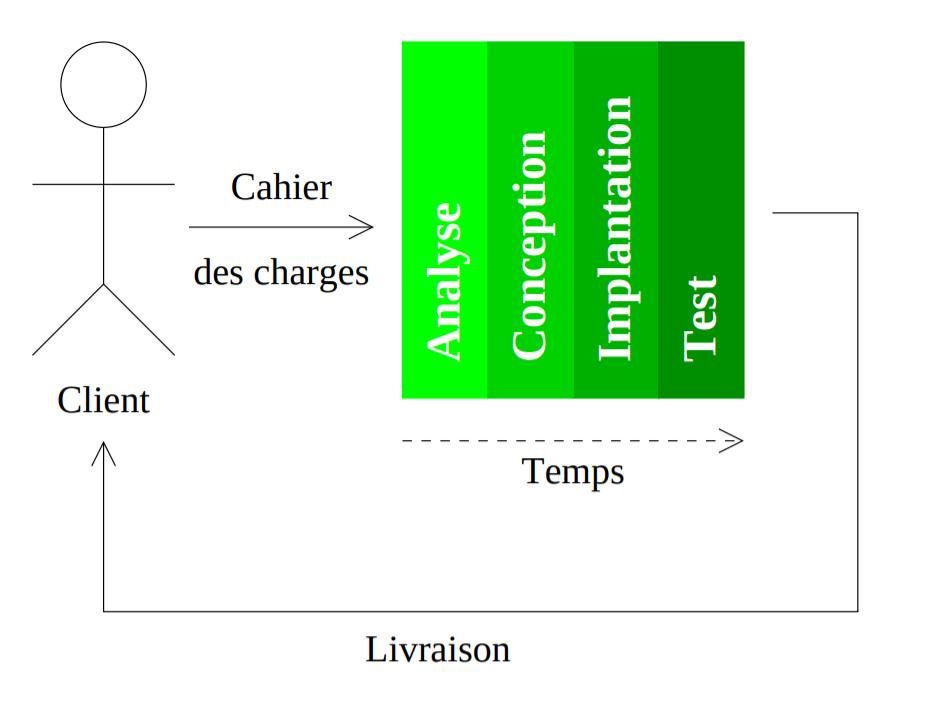
\includegraphics[width = 5in, height = 3in]{../images/analyse_conception.png}
\caption{Développement en cascade}
\end{figure}


\section{Langage de modélisation}
\subsection{UML}
\vspace{0.1in}
\hspace*{0.16in}
\textbf{U}nified \textbf{M}odeling \textbf{L}anguage ou langage de modélisation unifié est un langage de modélisation de développement à usage général dans le domaine du génie logiciel qui vise à fournir un moyen standard de visualiser la conception d’un système

\vspace{0.1in}

\begin{figure}[h]
\centering
    
\includegraphics[width = 2in, height = 0.95in]{../images/UMLlogo.png}
  \caption{Logo UML (Unified Modeling Language)}
\end{figure}

\newpage


\section{Les diagrammes utilisés}
\hspace*{0.16in}
Pour mieux concevoir notre application, nous avons besoin d’utiliser les trois types de diagrammes suivants :

\vspace{0.1in}

\begin{table}[h]
\begin{tabular}{|l|l|c|}
\hline
\rowcolor[HTML]{9B9B9B} 
\textbf{Diagramme}                                                       & \textbf{Objectifs}                                                                                                                                                                                                                                                                                                                                                                                                                    & \multicolumn{1}{l|}{\cellcolor[HTML]{9B9B9B}\textbf{Type}} \\ \hline
\rowcolor[HTML]{9698ED} 
\begin{tabular}[c]{@{}l@{}}Diagramme de cas\\ d'utilisation\end{tabular} & \begin{tabular}[c]{@{}l@{}}1. Identifier la fonctionnalité du système\\ 2. Il décrit l'interaction des personnes \\ ou du dispositif externe avec le système \\ en cours de conception.\\ 3. Il résume les relations entre les cas\\ d'utilisation, les acteurs et les systèmes.\end{tabular}                                                                                                                                         & Fonctionnel                                                \\ \hline
\rowcolor[HTML]{9698ED} 
Diagramme de composants                                                  & \begin{tabular}[c]{@{}l@{}}1. Il permet aux concepteurs d'applications\\ de vérifier que les fonctionnalités requises\\ d'un système sont mises en œuvre par les\\ composants, garantissant ainsi que le système\\ final sera acceptable.\\ 2. De plus, le diagramme des composants est un\\ outil de communication utile entre les parties\\ prenantes pour discuter, analyser ou améliorer\\ la conception du système.\end{tabular} & Statique                                                   \\ \hline
\rowcolor[HTML]{9698ED} 
Diagramme de déploiement                                                 & \begin{tabular}[c]{@{}l@{}}1. Décrire les composants matériels utilisés\\ dans les implémentations de systèmes ainsi que\\ les environnements d'exécution et les artefacts\\ déployés sur le matériel.\\ 2. Il permet de visualiser le système de\\ topologie du matériel, de modéliser les\\ éléments matériels physiques et la relation\\ de communication entre eux, et de planifier\\ l'architecture du système.\end{tabular}     & Statique                                                   \\ \hline
\end{tabular}
\caption{Les diagrammes utilisé}
\end{table}

\section{Diagramme de Cas d'utilisation}
\subsection{Définition}
\hspace*{0.16in}
Un diagramme de cas d'utilisation dans sa forme la plus simple est une représentation de l'interaction d'un utilisateur avec le système qui montre la relation entre l'utilisateur et les différents cas d'utilisation dans lesquels l'utilisateur est impliqué. Un diagramme de cas d'utilisation peut identifier les différents types d'utilisateurs d'un système et les différents cas d'utilisation et seront souvent accompagnés également d'autres types de diagrammes.

Les diagrammes de cas d'utilisation contiennent généralement :

\begin{itemize}
    \item Cas d'utilisation.
    \item Acteurs.
    \item Relations de dépendance, généralisation et association.
\end{itemize}

\hspace*{0.16in}
Comme tous les autres diagrammes, les diagrammes de cas d'utilisation peuvent contenir des notes et des contraintes.
\\
\hspace*{0.16in}
Les diagrammes de cas d'utilisation peuvent également contenir des packages, qui sont utilisés pour regrouper des éléments de votre modèle en blocs plus volumineux. Parfois, vous souhaiterez également placer des instances de cas d'utilisation dans vos diagrammes, en particulier lorsque vous souhaitez visualiser un système d'exécution spécifique.\textsuperscript{\cite{booch2005unified}}

\vspace{0.2in}

\begin{figure}[h]
\centering
    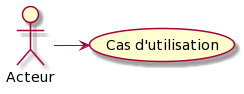
\includegraphics[width = 3.0in, height = 1.0in]{../images/usecaseEG.png}
    \caption{Exemple de cas d'utilisation}
\end{figure}

\subsection{Identifications des acteurs}
\hspace*{0.16in}
Avant d’entamer la présentation des diagrammes, il faut identifier les acteurs qui interagissent directement avec le système. Un acteur est une entité externe qui peut être un utilisateur humain, un dispositif matériel ou un autre système.
\\
Dans notre système on distingue deux acteurs principaux :

\begin{itemize}
    \item Administrateur : c’est lui qui va gérer les comptes clients ainsi que les chambres d’hôtel (Ajouter, Modifier et Supprimer).
    \item Clients : c'est lui qui va réserver ou bien consulter le site web afin d'authentifier.
\end{itemize}

\subsection{Identification des cas d’utilisation}

\newpage

\subsection{Diagramme de cas d’utilisation général}

\begin{figure}[h]
\centering
  \vspace{-0.1in}
    \centerline{\fbox{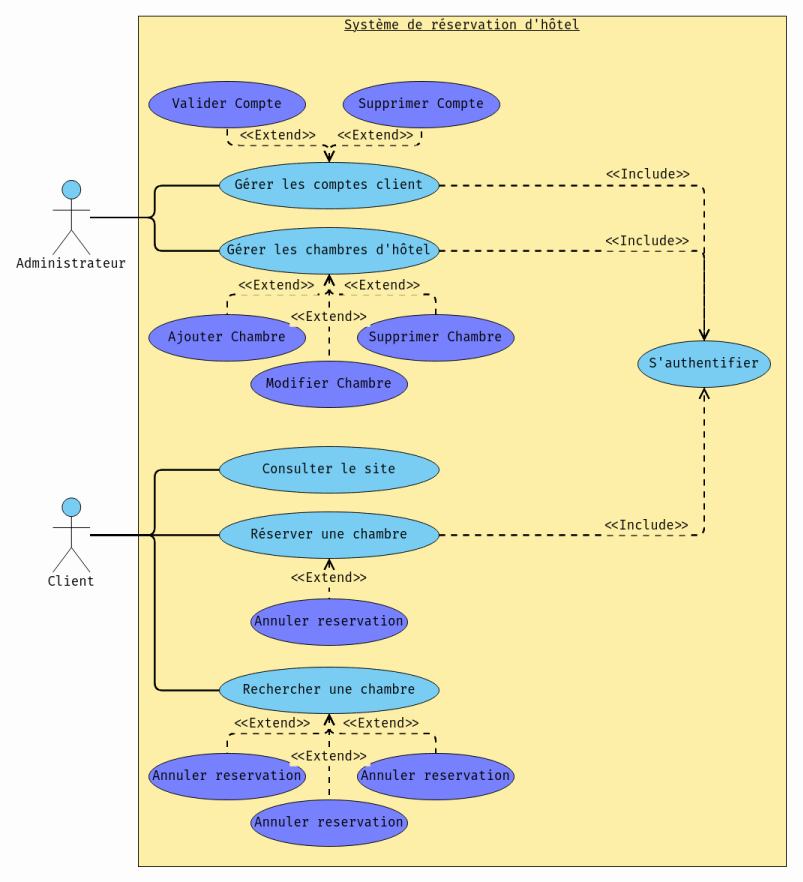
\includegraphics[width = 6.6in, height = 7in]{../images/UCD.png}}}
    \caption{Diagramme de cas d’utilisation général}
\end{figure}

\newpage

\section{Diagramme des composants}
\subsection{Définition}
\hspace*{0.16in}
Décrivent les composants du logiciel, leurs interfaces et leurs dépendances, les diagrammes de composants sont utiles pour les raisons suivantes :

\begin{itemize}
    \item Définition des aspects exécutables et réutilisables d'un système logiciel.
    \item Mise en évidence des problèmes de configuration logicielle à travers les relations de dépendance
    \item Représentation précise d'une application logicielle avant d'y apporter des changements ou des extensions.
\end{itemize}

\subsection{Diagramme des composants général}

\begin{figure}[h]
\centering
  \vspace{-0.1in}
    \centerline{\fbox{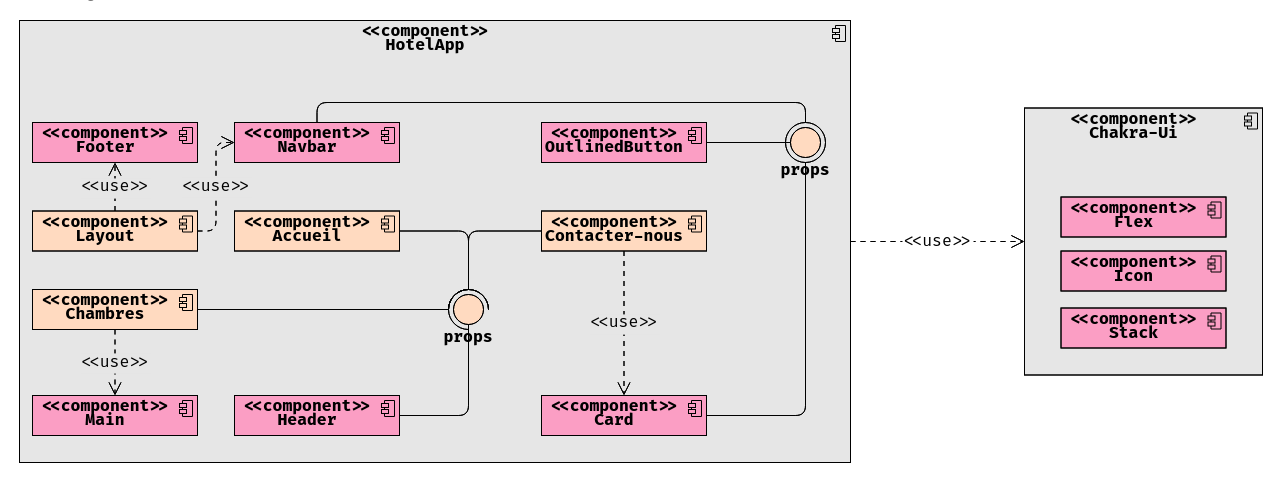
\includegraphics[width = 6.6in, height = 5.2in]{../images/components.png}}}
    \caption{Diagramme des composants général}
\end{figure}

\newpage

\section{Conclusion}
\hspace*{0.16in}
Dans ce chapitre, nous avons défini d’abord la signification de l’analyse et la conception avec les outils qu’on a utilisés pour réussir notre conception, ensuite nous sommes passés aux différents diagrammes là où nous avons expliqué notre solution en détail. 
\\
\hspace*{0.16in}
Cette étude nous a permis de définir la structure de l’application et cela aussi nous a facilité l’implémentation que vous verraient dans le chapitre suivant.

\newpage

\newpage

\vspace*{-0.2in}

\begin{center}
    {\color{Blue} \rule{5.5in}{1.4mm} }\\
    \vspace{0.1in}
    \scshape{\fontsize{34}{46}{\bfseries{\color{Blue}{Conclusion générale}}}}
    \\
    \vspace{0.5in}
\end{center}
\addcontentsline{toc}{chapter}{\vspace{-0.12in}\color{Blue}{Conclusion générale}}

\newpage

\bibliography{rapport}

\end{document}
